\documentclass[11pt]{article}

% parameters are fairly self-explanatory here, thankfully
\usepackage[width=7in,height=9.5in,top=0.75in,centering]{geometry}

% for math-ing
\usepackage{amsmath}
\usepackage{amssymb}


%%%%%% tables %%%%%%%%

\usepackage{array}
\renewcommand{\arraystretch}{1.5}
\setlength{\tabcolsep}{8pt}

%%%%%% plotting %%%%%%

\usepackage[dvipsnames]{xcolor}
\usepackage{tikz}
\usepackage{pgfplots}

\pgfplotsset{every axis/.append style={
                    axis x line=middle,    % put the x axis in the middle
                    axis y line=middle,    % put the y axis in the middle
                    axis line style={<->,color=black}, % arrows on the axis
                    xlabel={$x$},          % default put x on x-axis
                    ylabel={$y$},          % default put y on y-axis
            }}
            
 \pgfplotsset{compat=1.14} % sometimes, everything falls apart without this
 
 %\usepgfplotslibrary{fillbetween} %for shading between curves

%%%%%% commands %%%%%%

% exam heading; course name is first argument, exam information is second argument
\newcommand{\Heading}[2]{
    \fbox{
        {\Large\textbf{#1}}
        }
    \hfill
    \fbox{
        \begin{minipage}{0.2\textwidth}
            \begin{center}
            \textbf{#2}
            \end{center}
        \end{minipage}
    }
    \par\vspace{0.1in}}

% for being lazy while beautifying integrals
\newcommand{\dint}{\displaystyle\int}

% for being lazy while beautifying limits
\newcommand{\dlim}{\displaystyle\lim}

%%%%%% stuff %%%%%%

\usepackage{fancyhdr}

%\setcounter{page}{0} % first page is page 0

\parindent0pt % no indent

\fboxsep=0.25cm % little space in fbox border

%%%%%% BEGIN! %%%%%%%

\begin{document}

\pagestyle{fancy}

% record goals here to create sense of transparency

\fancyhead[l]{%
  \ifcase\value{page}
  % empty test for page = 0
  \or {}% 
  \or
  \or {\bf\color{ProcessBlue} F1: Lines \& Slope}% page=1
  \or {\bf\color{RoyalBlue} L1: Limits and Continuity}% page = 2
  \or {\bf\color{RoyalBlue} L2: Evaluating Limits Using Continuity and Forms}% page = 3
  \or {\bf\color{ForestGreen} D1: Meaning of a Derivative}% page = 4
  \or
  \else
  % Empty chead here!
  \fi
}

\thispagestyle{empty} % don't display that this is page 0

\Heading{MATH 1190/1210 Survey of Calculus I}{Knowledge Checkpoint 1\\Growth-Based\\Fall 2025}

\vspace{0.1in}

\textbf{Name} \hrulefill \, \begin{minipage}{0.16\textwidth}\begin{center}\textbf{UVA ID\\ (e.g. hdj4nd)} \end{center}\end{minipage}\hrulefill\\

\begin{minipage}{0.2\textwidth}\begin{center}\textbf{Course \&\\ Section Number} \end{center}\end{minipage} \hrulefill\,\,\textbf{Date} \hrulefill  \\

\hrulefill
\paragraph*{Course \& Section Numbers:}

{\small
\begin{center}
\begin{tabular}{| c | c | c | c | c |}
\hline
%
\begin{minipage}{0.12\textwidth}\begin{center}
1190-100\\
J. Rolf\\
(11:00 AM)
\end{center}\end{minipage}
&
\begin{minipage}{0.12\textwidth}\begin{center}
1190-200\\
J. Rolf\\
(9:30 AM)
\end{center}\end{minipage}
&
\begin{minipage}{0.12\textwidth}\begin{center}
1210-100\\
Mikhail\\
(8 AM)
\end{center}\end{minipage}
&
\begin{minipage}{0.12\textwidth}\begin{center}
1210-200\\
Raul\\
(9:30 AM)
\end{center}\end{minipage}
&
\begin{minipage}{0.12\textwidth}\begin{center}
1210-300\\
Sherman\\
(11 AM)
\end{center}\end{minipage}
\\
%
\hline
%
\begin{minipage}{0.12\textwidth}\begin{center}
1210-400\\
Sherman\\
(12:30 PM)
\end{center}\end{minipage}
&
\begin{minipage}{0.12\textwidth}\begin{center}
1210-500\\
Michael\\
(2 PM)
\end{center}\end{minipage}
&
\begin{minipage}{0.12\textwidth}\begin{center}
1210-600\\
J. Bowling\\
(3:30 PM)
\end{center}\end{minipage}
&
\begin{minipage}{0.12\textwidth}\begin{center}
1210-700\\
Josh\\
(9:30 AM)
\end{center}\end{minipage}
&
\begin{minipage}{0.12\textwidth}\begin{center}
1210-800\\
Mason\\
(2 PM)
\end{center}\end{minipage}
\\
%
\hline
%
\begin{minipage}{0.12\textwidth}\begin{center}
1210-900\\
Caelan\\
(3:30 PM)
\end{center}\end{minipage}
&
\begin{minipage}{0.12\textwidth}\begin{center}
1210-920\\
Caelan\\
(5 PM)
\end{center}\end{minipage}
&
\begin{minipage}{0.12\textwidth}\begin{center}
1210-940\\
Mitchell\\
(10 AM)
\end{center}\end{minipage}
&
\begin{minipage}{0.12\textwidth}\begin{center}
1210-950\\
Mitchell\\
(11 AM)
\end{center}\end{minipage}
&
\begin{minipage}{0.12\textwidth}\begin{center}
1210-960\\
Mitchell\\
(noon)
\end{center}\end{minipage}
\\
\hline
\end{tabular}
\end{center}

}

{%\small

\paragraph*{Instructions:}

\begin{itemize}
    
    \item The regular time allowed for completing this assessment is \fbox{$40$} minutes.
    %\item This assessment is out of 50 points.\\
    \item This assessment contains one single-part or multi-part problem for each of the following targets: {\bf\color{ProcessBlue}F1}, {\bf\color{RoyalBlue}L1}, {\bf\color{RoyalBlue}L2}, {\bf\color{ForestGreen}D1}.
    \item On each problem, you will receive a score of Exceeds Expectations (5), Proficient (4), Almost (3), Developing (2), Emerging (1), or Not Yet (0). {\bf Please do not interpret your score as a percentage.}
    %\item You will have opportunities to reassess on the targets appearing on this assessment after the next {\bf 2} assessments.\\
    \item You may NOT use calculators, dictionaries, notes, phones, or any other kind of aid.
    \item Please write neatly. What cannot be read, cannot be graded.
    \item Carefully work out each problem and clearly indicate your final answer to every problem.
    \item Throughout, give the most descriptive answer possible. \textbf{For instance, ``DNE" will not be accepted when ``$=\infty$" is applicable.}
    %\item Please provide the most specific answer possible. For instance, if a limit does not exist because it goes to $\infty$ or $-\infty$, then specify this.
    \item Please use the methods discussed up to this point in the course. For example, any work based on l'H\^opital's Rule will not receive credit.
    \item \textbf{All work must be shown unless otherwise specified.} Partial credit will not be given if appropriate work is not shown.
    \item In particular, {\bf any answer appearing with no justification will receive no credit regardless of whether the answer was correct}, unless otherwise specified.
    \item Please first respond to the prompts on which you feel most proficient, then respond to others later.
    \item This booklet is printed double-sided. It contains 8 pages and 4 numbered problems.
    \end{itemize}
    
    }

\vfill


%%%%%%%%%
\newpage

This page is left blank intentionally.\\

Use this page if you need additional space to write your solutions to any problem. \\

If you wish this page graded, you must refer to this page on \textbf{the original page} of the problem. Otherwise, your grader will NOT consider your work on this page.

\newpage%
%%%%%%%%%


\begin{enumerate}

%%%%%%%%%%%%%%%%%%%%%%%%%%%%%%%%%%%%%%%%%%%%%%%%%%%%%
%%%%%%%%%%% BEGIN PROBLEM F1 %%%%%%%%%%%%%%%%%%%%%%%%
%%%%%%%%%%%%%%%%%%%%%%%%%%%%%%%%%%%%%%%%%%%%%%%%%%%%%

\item Below is a chart showing estimates of the population of Whitetail Deer (\textit{Odocoileus virginianus}) in the US since 1900.

\begin{center}
    
\includegraphics[scale=0.7]{Fall 2025/KCs/KC1/deer_population.png}
\end{center}


%In 2005, the total value of US imports is 1700 billion dollars. In 2020, the total value of US imports is 2300 billion dollars. 
%
%Add table!!!!!

\begin{enumerate}
    \item Estimate the net change of the deer population from 1900 to 2000. Make sure to include units in your final result.

    \vfill

    \item Estimate the average rate of change of the deer population from 1900 to 2000. Again, make sure to include units in your final result.

    \vfill

    \item Use a sentence or two to explain the meaning of the average rate of change \textbf{in the context of this scenario}. 
    
    Do NOT use average rate of change or slope in your explanation.

    \vfill

    %\item Based on the information given, what do you think the total value of US imports in 2021 would be?
\end{enumerate}


%%%%%%%%%%%%%%%%%%%%%%%%%%%%%%%%%%%%%%%%%%%%%%%%%%%%%
%%%%%%%%%%% END PROBLEM F1 %%%%%%%%%%%%%%%%%%%%%%%%%%
%%%%%%%%%%%%%%%%%%%%%%%%%%%%%%%%%%%%%%%%%%%%%%%%%%%%%

\newpage

%%%%%%%%%%%%%%%%%%%%%%%%%%%%%%%%%%%%%%%%%%%%%%%%%%%%%
%%%%%%%%%%% BEGIN PROBLEM L1 %%%%%%%%%%%%%%%%%%%%%%%%
%%%%%%%%%%%%%%%%%%%%%%%%%%%%%%%%%%%%%%%%%%%%%%%%%%%%%

\item Sketch the graph of a function $f(x)$ defined on the interval $[-1,5]$ which satisfies the following constraints:

\begin{enumerate}
    \item The one-sided limit $\displaystyle\lim_{x\to 0^+}f(x)$ does not exist.
    \item $\displaystyle\lim_{x\to 2}f(x) = 3$.
    \item $f(x)$ has a jump discontinuity at $x=4$.
    \item $f(x)$ is discontinuous only at $x=0$ and $x=4$.
\end{enumerate}
\vspace{2cm}
\begin{center}
    \begin{tikzpicture}[scale=1]
    \begin{axis}[
        %    axis y line = left,
        %    axis x line = bottom,
            xlabel={$x$},
            xtick       = {-1,1,2,3,4,5},
            xticklabels = {$-1$,$1$,$2$,$3$,$4$,$5$},
            ylabel={$f(x)$},
            ytick       = {1,2,3,4,5},
            yticklabels = {$1$,$2$,$3$,$4$,$5$},
            samples     = 160,
            domain      = -1.5:5.5,
            restrict y to domain=-2.5:2.5,
            xmin = -1.5, xmax = 5.5,
            ymin = -0.5, ymax = 5.5,
            grid=both, grid style=dashed,
            width=5.5in, height=5in
          ]
          % \addplot[ultra thick,blue,<-, domain=-4:-2] {(1/4)*(x+2)^2};
          % \addplot[ultra thick,blue,->, domain=-2:2] {-1/(x^2+x-6)-0.25};
          % \addplot[ultra thick,blue,<-, domain=2:5] {2/(x^2+x-6)};
          % \filldraw[fill=white,ultra thick] (-2,0) circle (2.5pt);
          % \filldraw (-2,2) circle (2.5pt);
          %\node at (-2,2.5) {\fbox{C}};
    \end{axis}
    \end{tikzpicture} 
\end{center}
\vfill

%%%%%%%%%%%%%%%%%%%%%%%%%%%%%%%%%%%%%%%%%%%%%%%%%%%%%
%%%%%%%%%%% END PROBLEM L1 %%%%%%%%%%%%%%%%%%%%%%%%%%
%%%%%%%%%%%%%%%%%%%%%%%%%%%%%%%%%%%%%%%%%%%%%%%%%%%%%

\newpage

%%%%%%%%%%%%%%%%%%%%%%%%%%%%%%%%%%%%%%%%%%%%%%%%%%%%%
%%%%%%%%%%% BEGIN PROBLEM L2 %%%%%%%%%%%%%%%%%%%%%%%%
%%%%%%%%%%%%%%%%%%%%%%%%%%%%%%%%%%%%%%%%%%%%%%%%%%%%%

\item Evaluate the following limits using continuity or form.

If you use continuity to evaluate a limit, to receive full credit, please provide sufficient explanation for why continuity can be used, including why the given function is continuous at the given point.

If you use form to evaluate a limit, to receive full credit, please list the form and show all steps. 

% DJ's wording: For each limit below, first find the form of the limit, then find the value of the limit. If the given function is continuous at the target, then you may simply write ``n/a" for the form. Show complete work - using mathematics and/or words - to accompany your answers.

\begin{enumerate}
    \item $\lim\limits_{x\to 0}\dfrac{1}{(x-1)^2}$

    % It's okay to say $x=-2$ is in the domain as the explanation

    \vfill

    \item $\lim\limits_{x\to 1}\dfrac{1}{(x-1)^2}$

    \vfill

    \item $\lim\limits_{x\to \infty}\dfrac{1}{(x-1)^2}$

    \vfill
\end{enumerate}

%%%%%%%%%%%%%%%%%%%%%%%%%%%%%%%%%%%%%%%%%%%%%%%%%%%%%
%%%%%%%%%%% END PROBLEM L2 %%%%%%%%%%%%%%%%%%%%%%%%%%
%%%%%%%%%%%%%%%%%%%%%%%%%%%%%%%%%%%%%%%%%%%%%%%%%%%%%

\newpage

%%%%%%%%%%%%%%%%%%%%%%%%%%%%%%%%%%%%%%%%%%%%%%%%%%%%%
%%%%%%%%%%% BEGIN PROBLEM D1 %%%%%%%%%%%%%%%%%%%%%%%%
%%%%%%%%%%%%%%%%%%%%%%%%%%%%%%%%%%%%%%%%%%%%%%%%%%%%%

\item  The following graph models the speed $v(t)$ of a sprinter $t$ second after they start running, where $v(t)$ is measured in meters per second.

% The figure below shows the power output, $p(w)$ (in watts), of a wind turbine as a function of wind speed $w$ (in m/sec). 

\begin{center}
    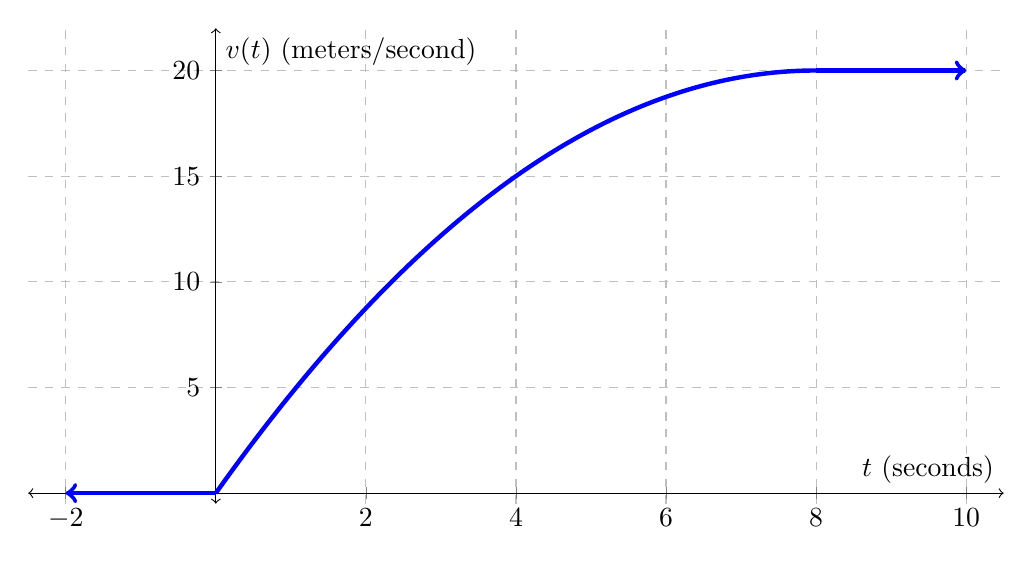
\begin{tikzpicture}[scale=1]
    \begin{axis}[
        %    axis y line = left,
        %    axis x line = bottom,
            xlabel={$t$ (seconds)},
            xtick       = {-2,2,4,6,8,10},
            xticklabels = {$-2$,$2$,$4$,$6$,$8$,$10$},
            ylabel={$v(t)$ (meters/second)},
            ytick       = {5,10,15,20},
            yticklabels = {$5$,$10$,$15$,$20$},
            samples     = 160,
            domain      = -2.5:10.5,
            restrict y to domain=-0.5:22,
            xmin = -2.5, xmax = 10.5,
            ymin = -0.5, ymax = 22,
            grid=both, grid style=dashed,
            width=5.5in, height=3in
          ]
          \addplot[ultra thick,blue,<-, domain=-2:0] {0};
          \addplot[ultra thick,blue, domain=0:8] {-.3125*(x-8)^2+20};
          \addplot[ultra thick,blue,->, domain=8:10] {20};
          % \addplot[ultra thick,blue,<-, domain=-4:-2] {(1/4)*(x+2)^2};
          % \addplot[ultra thick,blue,->, domain=-2:2] {-1/(x^2+x-6)-0.25};
          % \addplot[ultra thick,blue,<-, domain=2:5] {2/(x^2+x-6)};
          % \filldraw[fill=white,ultra thick] (-2,0) circle (2.5pt);
          % \filldraw (-2,2) circle (2.5pt);
          %\node at (-2,2.5) {\fbox{C}};
    \end{axis}
    \end{tikzpicture} 
\end{center}


% Embed units into statement above

\begin{enumerate}    
    \item Explain the meaning in this context of the equality
    \[
        \lim_{h\to 0}\frac{v(4+h) - v(4)}{h} = 2.5.
    \]
    To receive full credit, please include units for all quantities discussed, and do not include any mathematical terms such as ``limit" or ``instantaneous rate of change".

    \vfill

    \item According to this model, for what time $t_0$ does \ \ 
    \(
        \displaystyle\lim_{h\to 0}\frac{v(t_0+h) - v(t_0)}{h}
    \)
    \ \ not exist? Explain.

    \vfill
\end{enumerate}


%%%%%%%%%%%%%%%%%%%%%%%%%%%%%%%%%%%%%%%%%%%%%%%%%%%%%
%%%%%%%%%%% END PROBLEM D1 %%%%%%%%%%%%%%%%%%%%%%%%%%
%%%%%%%%%%%%%%%%%%%%%%%%%%%%%%%%%%%%%%%%%%%%%%%%%%%%%

\newpage

This page is left blank intentionally.\\

Use this page if you need additional space to write your solutions to any problem. \\

If you wish this page graded, you must refer to this page on \textbf{the original page} of the problem. Otherwise, your grader will NOT consider your work on this page.

\newpage

This page is left blank intentionally.\\

Use this page if you need additional space to write your solutions to any problem. \\

If you wish this page graded, you must refer to this page on \textbf{the original page} of the problem. Otherwise, your grader will NOT consider your work on this page.

\end{enumerate}

\end{document}